\documentclass[]{article}
\usepackage[utf8]{inputenc}
\usepackage[T1]{fontenc}
\usepackage{amsmath}
\usepackage{amsfonts}
\usepackage{amssymb}
\usepackage{graphicx}
\usepackage{amsthm}
\usepackage{mathtools} 
\usepackage{tikz}
\usepackage{hyperref}
\usepackage{caption}
\usepackage{subcaption}
\usepackage{cjhebrew}
\usepackage{url}
\usepackage{placeins}
\usepackage{flafter}
\usepackage{comment}
\usepackage{ulem}

\newtheorem{theorem}{Theorem}[section]
\newtheorem{corollary}{Corollary}[theorem]
\newtheorem{lemma}[theorem]{Lemma}
\newtheorem{example}[theorem]{Example}
\newtheorem{conjecture}[theorem]{Conjecture}

\theoremstyle{definition}
\newtheorem{definition}{Definition}[section]
\newtheorem{notation}{Notation}[section]

\theoremstyle{remark}
\newtheorem*{remark}{Remark}

\newenvironment{sproof}{%
	\renewcommand{\proofname}{Proof Sketch}\proof}{\endproof}

\DeclarePairedDelimiter\abs{\lvert}{\rvert}%
\DeclarePairedDelimiter\norm{\lVert}{\rVert}%

\newcommand{\interior}[1]{%
	{\kern0pt#1}^{\mathrm{o}}%
}

\newcommand{\diag}[1]{%
	\text{Diag}(#1)%
}

\newcommand{\R}{\mathbb{R}}
\newcommand{\C}{\mathbb{C}}
\newcommand{\NN}{\mathbb{N}}

\newcommand{\M}{\mathcal{M}}
\newcommand{\N}{\mathcal{N}}
\newcommand{\OO}{\mathcal{O}}
\newcommand{\B}{\mathcal{B}}
\newcommand{\bb}{\boldsymbol{b}}
\newcommand{\A}{\Lambda}
\newcommand{\LL}{\mathcal{L}}
\newcommand*\colvec[2]{\begin{pmatrix} #1 \\ #2\end{pmatrix}}
\newcommand{\ivec}{(\text{CT})\cap(\text{NCR})}
%opening
\title{Reproducing a result from the paper "Retinal Prosthetic Vision Simulation:
	Temporal Aspects" by Avraham et.al}
\author{Omer Rosler}

\begin{document}

\maketitle


\begin{abstract}
	
We try to reproduce one of the claims in paper \cite{main_paper} that there is a "contour vision" for the simulated prosthetic.  The code and data of our results is found in \cite{our_code}. Our results mostly suggest it is true (under some restrictions), and we refine the claim by the author.
	
\end{abstract}

\section{Summary of the paper}

This paper \cite{main_paper} is in the field of prosthetic vision. Certain types of degenerative blindness can be treated with prosthetic devices. The prosthetic architecture studied in this paper consists of two parts -  a mounted camera, and an electrode array mounted inside the retina. Each electrode emits an electric pulse at a steady pace, (with frequencies of 6, 10, or 30 Hz for the main prosthetic simulated in the paper, the Argus II). This has the effect of seeing a spot of light in the patient's field of view. This white light is called a "phosphene" in the literature. Using an array of these electrodes enables "pattern vision".

This paper (along with the code \cite{paper_code}) contains simulations of this prosthetic vision. The main novelty of the paper is a simulation architecture that includes temporal effects. Using this new simulation technique, it analyzed the temporal effects and reached several conclusions regarding user training and the planning and development of future prosthetic devices.

\subsection{Temporal effects}
This paper explores two temporal effects, we quote the definitions from the paper:

\begin{enumerate}
	\item Persistence: It was found that some subjects perceived phosphenes that lasted as long as 8 s after the end of the stimulation. 
	\item Perceptual fading: With continuous stimulation, phosphenes begin to fade out after a variable duration up to 10 s, over a fading out
	duration for individual users ranges from 0.5 s to more than 60 s
\end{enumerate}

These are measurable quantities, and they vary between users (and presumably between prosthetic architectures, but this was not described in this paper). The persistence time in seconds is described by PER, and the perceptual fading onset is described by PFO (the duration of continuous stimulation until the phosphene begin to fade, the fading time duration is a separate parameter called PFD).\\

\begin{remark}
	I wanted to test the prevalence of the PFD (perceptual fading duration) on the results as well. However, it seems there is a bug in the simulation code, where the PFD provided by the user is being ignored in the heart of the model. Therefore I use the preset value (2 seconds) throughout my analysis.
\end{remark}

The paper runs simulations to understand the effects of these "parameters" on the perception of the user. \\

The other perceptual effects discussed in the paper include "flickering" (3.1), "the stroboscopic effect" (3.2), "smearing" (3.3), and "contour vision" (3.6), we will focus only on the last one.
\subsection{The Testable Claim}
The claim I chose to try and reproduce is in section 3.6 : Exploiting persistence, by using "scanning head movements" we can reproduce the contour of a static object {\bf after} the perceptual fading started. \\
In other words, we can counteract the negative effect of perceptual fading using persistence. {\it "Two wrongs \sout{don't} make a right."}

To mimic head movements that scan a static object, the paper "inverted the perspective" i.e., created videos of the objects moving in direction opposite to the movement. 
\begin{remark}
	One may argue this is a wrong approach, as the object is in 3D, and one needs to apply projective transformations to change perspective. However, due to the low resolution of the prosthetic, the claimed contour vision works only for close and large objects (relative to the field of view). In this case, the difference between the approaches is negligible. The author addressed this fact indirectly in the "future research" section which suggested using virtual reality.
\end{remark}
The original paper ran simulations on very specific videos using very specific values for the temporal parameters. The claim is based on "seeing" the result with our eyes (figure 9 in the paper). Originally, I thought this claim to be robust, but after examining the videos used more closely, it seems to be less so. \\
Therefore, in order to reproduce this claim, I first needed to quantify it.

The "input data" is a video of an object scanned using head movements, and the result is a number representing the similarity between the contour of the object and the apparent contour at the end of the simulated video.
\section{Methods}
\subsection{Quantifying the claim}
The code available at \cite{paper_code} generates a simulation of what the patient sees with the prosthetic. By extracting the frames at the end, we compare these to the original video (before the movement).
To obtain a quantifiable result, we aimed to extract the contour and use a standard shape-matching algorithm. Specifically, I use the `matchShapes` function from the python OpenCV library \cite{opencv_library} , with the chosen method being `CV\_CONTOURS\_MATCH\_I2` which is more suitable for noisy conditions (as is the case here due to "persistence").

\begin{figure}[h] % 'h' means here, try to place the figure where it is in the text
	\centering
	
	\begin{subfigure}{0.45\textwidth}
		\centering
		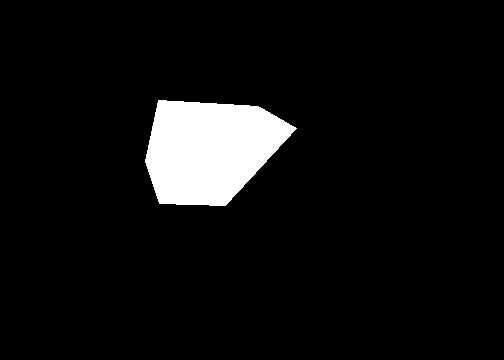
\includegraphics[width=\textwidth]{first_orig_frame.png}
		\caption{The image captured by the camera}
		\label{compare_images:orig}
	\end{subfigure}
	\hfill
	\begin{subfigure}{0.45\textwidth}
		\centering
		
\includegraphics[width=\textwidth]{first_simulated_frame.png}
		\caption{The image simulated}
		\label{compare_images:analysed}
	\end{subfigure}
	
	\caption{Comparison of real object and simulation (static)}
	\label{fig:image_comparison}
\end{figure}

The main problem is that I can't  extract the contours directly from the phosphene image. Therefore I applied some standard image processing functions (morphological transformation) to extract an approximate contour.
First we apply "closing" which is dilation followed by erosion. This removes the tiny holes which are due to the distance between phosphenes in the image. Next, we apply "skeletonization" to recover the shape (we used the open source python library \cite{scikit-image}). This results in a thin contour-like shape which is disconnected and branched. We then merge the disconnected pieces as described in \cite{stackoverflow}. This final result is a convex hull that approximates the shape.


\begin{figure}[h] % 'h' means here, try to place the figure where it is in the text
	\centering
	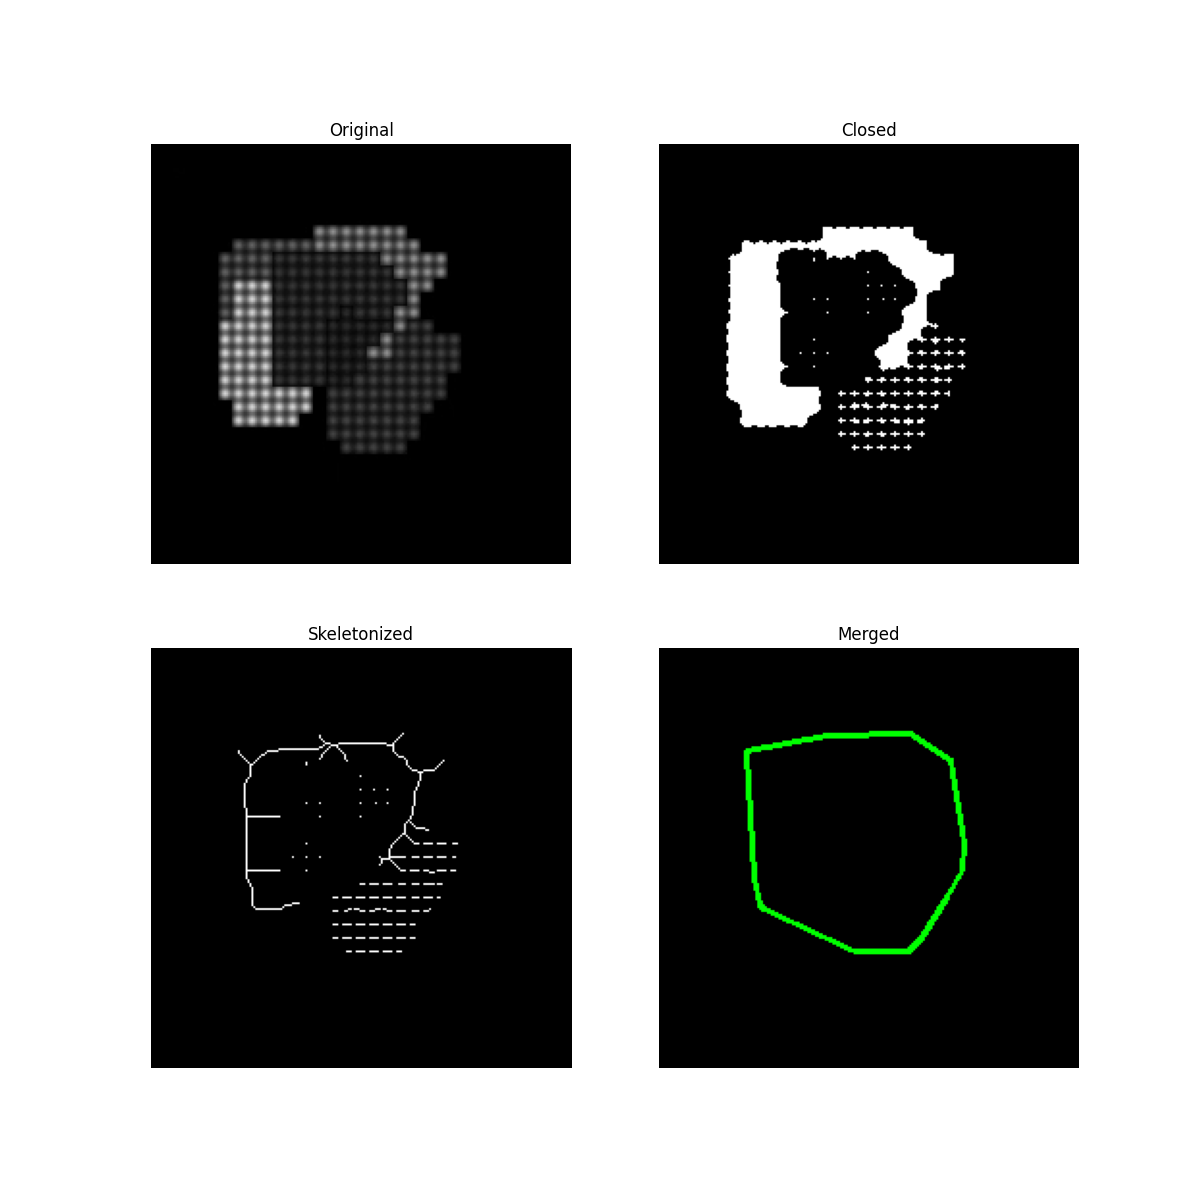
\includegraphics[width=0.8\textwidth]{compare_pipeline.png}
	\caption{The process steps}
	\label{fig:example_image}
\end{figure}

\subsection{Choosing the input videos}
Using the apparatus described above, we input videos of objects being scanned and obtain a metric describing the accuracy of contour detection. \\

This is a very open-ended dataset, therefore we need to decide what objects to test. My approach is to try and refute the claim of the author. Therefore I developed a list of conjectures regarding potential biases in the videos used in the paper. The conjectures lead to "useful" datasets. 
The conjectures are:
\begin{enumerate}
	\item The shapes used were too symmetrical.
	\item The directions of the head movement are perpendicular to the contour of the object.
	\item There is no delay between the perceptual fading onset and the start of the head movements. In reality, there would be a small delay, or maybe even premature movement.
	
	\item The contour vision is most prominent when the PFO and PER are close to each other.

\end{enumerate}
To test the first three conjectures, I created a dataset of videos of objects which are being scanned with the following parameters:
\begin{enumerate}
	\item Randomized shape of the object
	\item Randomized {\it delayed or premature} start of the movement (relative to the Perceptual Fading Duration)
	\item Randomized directions and speed of movement
\end{enumerate}
To test the fourth claim, I ran the simulation code with different values for the PFO and PER.

\begin{remark}
	I had trouble determining the actual speed used by the author. The paper cites a certain range in section 2.3, but the videos used in the simulation follow a much lower speed. \\
	In our simulations, we used the value cited in the paper.
	
	This does not affect the validity of our claim, as these movements simulate head scanning of an object. Increasing the speed induces a similar effect to moving the object further away. Therefore, even if our code used an incorrect speed, the results would still be applicable to more distant objects, and remain meaningful.
\end{remark}

\section{Results}
First we note the result of the matching algorithm is a number that is interpreted as "smaller" the better match. We don't have absolute meaning, but we can still compare it.

We now list all parameters used:
The simulation parameters are PER and PFO.
\subsection{Quantifying the original data}
We want to quantify the original 3 videos used by the author, i.e. figure 9. This is done by setting PER to 0 or 3 and PFO to 0.5. The result was as follows, for PER=0 the match score was the special value '1.7976931348623157e+308' which indicates the shapes were drastically different. For the value PER=3 we got the following results:
\begin{table}[h!]
	\centering
	\begin{tabular}{|c|c|c|}
		\hline
		Ellipse & Rectangle & Triangle \\
		\hline
		12.884957614701374 & 0.08348188961649206 & 20.25174440803744  \\
		\hline
	\end{tabular}
	\caption{Results of the original data}
	\label{fig:original_results}
\end{table}

The first two conjecture seems to explain the fact the rectangle is a very good match.
\subsection{Quantifying the generated data}
We put the result along with the suite of parameters into a python "pandas" database and performed some queries, described in the "data\_analysis.py" file. A sanity check is that every time the match completely failed (i.e.\ no contour detection at all) was when PER was zero, i.e. no persistence. 
There were a number of queries with graphs not shown, but are in the repository.

We analyzed the data, first per video (to compare the simulation parameters):

For most of the videos, higher PER was directly correlated with a better match. For others this ratio was more complex.

There was no apparent correlation between higher PFO and the match score.

The scale of the results for each video is the same (except for the case PER=0.0), which means the randomization process made no significant difference. This refutes completely conjecture 3 and only partially conjecture 2.

The fourth conjecture is also blatantly false.

\begin{figure}[h] % 'h' means here, try to place the figure where it is in the text
	\centering
	\begin{subfigure}{0.45\textwidth}
		\centering
		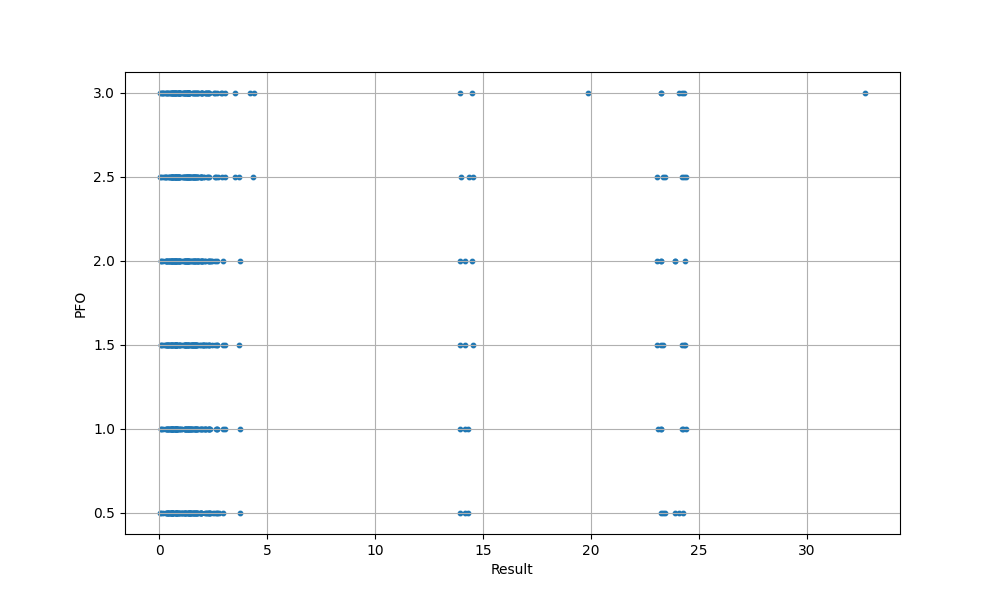
\includegraphics[width=\textwidth]{QueryPFO.png}
		\caption{The relation between PFO and the match}
		\label{graphs:pfo}
	\end{subfigure}
	\hfill
	\begin{subfigure}{0.45\textwidth}
		\centering
		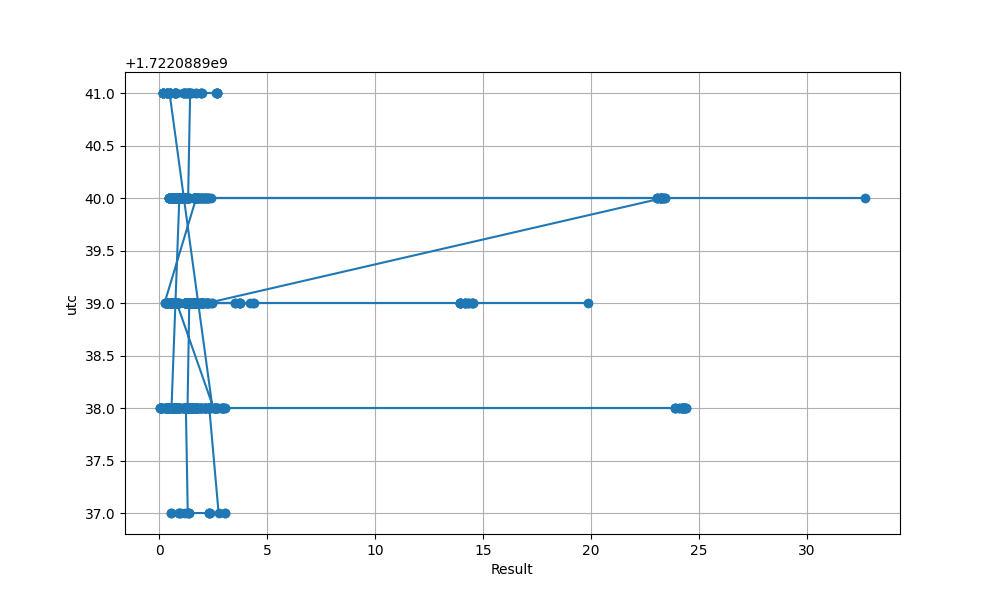
\includegraphics[width=\textwidth]{QueryScaleOfMatch.png}
		\caption{Proving randomization didn't matter}
		\label{graphs:random}
	\end{subfigure}
	\vfill
	\begin{subfigure}{0.45\textwidth}
		\centering
		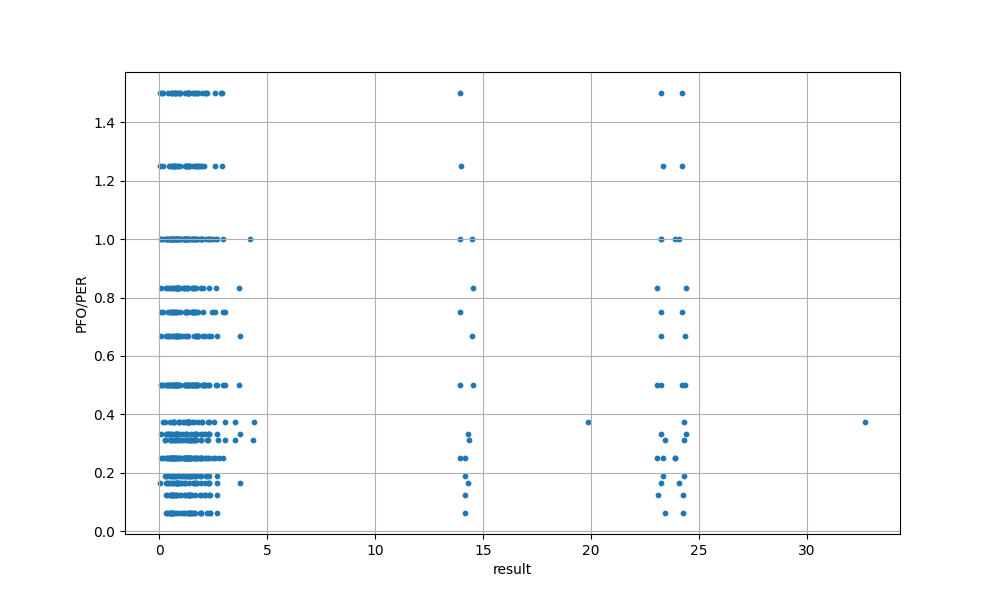
\includegraphics[width=\textwidth]{QueryRatio.png}
		\caption{Conjecture 4 is false}
		\label{graphs:conj4}
	\end{subfigure}
	\hfill
	\begin{subfigure}{0.45\textwidth}
		\centering
		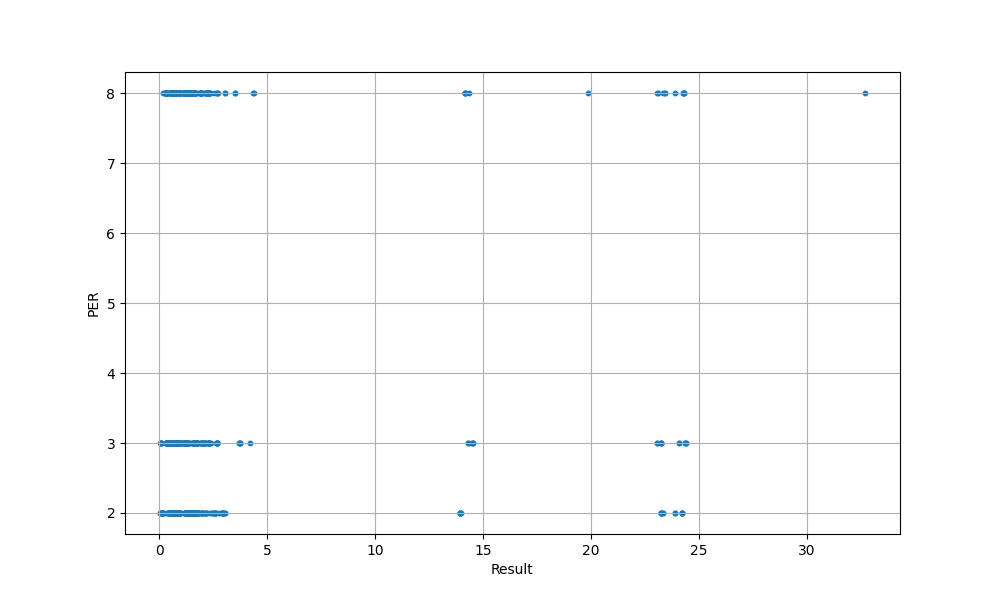
\includegraphics[width=\textwidth]{QueryPER.png}
		\caption{Higher PER correlates with better match}
		\label{graphs:PER}
	\end{subfigure}
	\caption{Results}
	\label{fig:results_graphs}
\end{figure}
There is still an unexplained smaller number of videos with very high match scores. We do not understand this wholly and this needs further analysis. 
\section{Conclusions}
Most importantly, the shape we want to look at matters most. 

We didn't disprove the second conjecture wholly. There coulb be a bias towards preferred directions of movement. We can definitely accept this, as the directions of movements are chosen by the user, and the training would be to choose these directions based on the perception of the object before the PFO.

We eve
In fact, we proved the conjecture true for most temporal parameters and refined the conjecture (without proving it completely, this needs further analysis):

\begin{conjecture}
To achieve contour vision of an object, the user should use head scanning motions in directions perpendicular to the most prominent direction in the convex hull.
\end{conjecture}


\bibliographystyle{plain}
\bibliography{refs} % Entries are in the refs.bib file
\end{document}
